\documentclass[12pt]{article}

% packages
\usepackage{setspace}
\usepackage{array}
\usepackage[margin=0.75in]{geometry}
\usepackage{amsmath,bm}
\usepackage{amssymb}
\usepackage{bbold}
\usepackage{physics}
\usepackage{xcolor}
\usepackage{indentfirst}
\usepackage{enumerate}
\usepackage{mathtools}
\usepackage{fancyhdr}
\usepackage{hyperref}

\newenvironment{changemargin}[2]{%
\begin{list}{}{%
\setlength{\topsep}{0pt}%
\setlength{\leftmargin}{#1}%
\setlength{\rightmargin}{#2}%
\setlength{\listparindent}{\parindent}%
\setlength{\itemindent}{\parindent}%
\setlength{\parsep}{\parskip}%
}%
\item[]}{\end{list}}

\allowdisplaybreaks

\title{Project 1: Unsupervised Machine Learning for Chemistry Data using Restricted Boltzmann Machines}
\date{}

\begin{document}

\maketitle

\subsection*{Before you start}

At this point, you'll have learned about some machine learning and its applications. This project will guide you through using a machine learning algorithm -- the Restricted Boltzmann machine (RBM) -- on molecular data. If you want some more exposure before you begin your tasks, supplemental reading on RBMs can be found \href{https://qucumber.readthedocs.io/en/stable/_static/RBM_tutorial.pdf}{here}, and a guide on training RBMs on a dummy dataset can be found in \texttt{RBM\_train\_dummy\_dataset.ipynb}. The base RBM code is located in \texttt{RBM\_helper.py}. We've intentionally left it to be pretty bare-bones and easy to use.

If you feel that you are very comfortable with RBMs and how they work, feel free to skip right to your tasks for Week 1!

\subsection*{Data science motivation?}

Data-compression is a central problem in science; scientists are always trying to figure out ways to represent things in a more efficient, compact package. 
It turns out that machine learning is one of the best tools out there for the job.
In the data science and machine learning community, the Modified National Institute of Standards and Technology (MNIST) database is arguably the most important benchmark database for machine learning algorithms. 
The database consists of hand-written digits like in Fig.~\ref{fig:MNIST_digits}. 
A machine learning algorithm reads in all of these hand-written digits as binary (0's and 1's) data, assigning a 0 to pixels of the image that are white and a 1 to pixels of the image that are black. 
After the machine learning algorithm has trained itself on this massive data set of hand-written digits, it offers itself as a compact ``digit generator''; a small file containing all the information required in order to generate \textit{new} instances of hand-written digits (i.e. hand-written digits that look like a real human drew them, but actually a machine generated!). See Fig.~\ref{fig:MNIST_ML}. 

\begin{figure}
    \begin{center}
        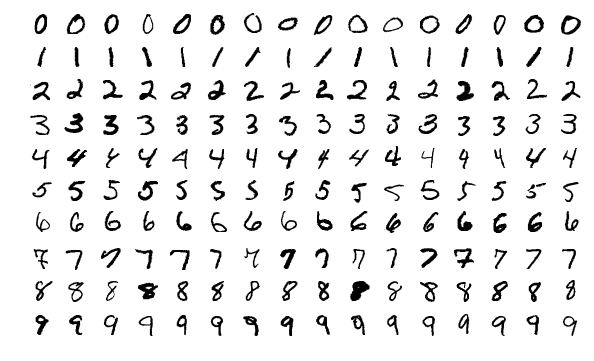
\includegraphics[width=0.5\linewidth]{../figures/MnistExamples.png}
    \end{center}
    \caption{Examples of hand-written digits in the MNIST database.}
    \label{fig:MNIST_digits}
\end{figure}

\begin{figure}
    \begin{center}
        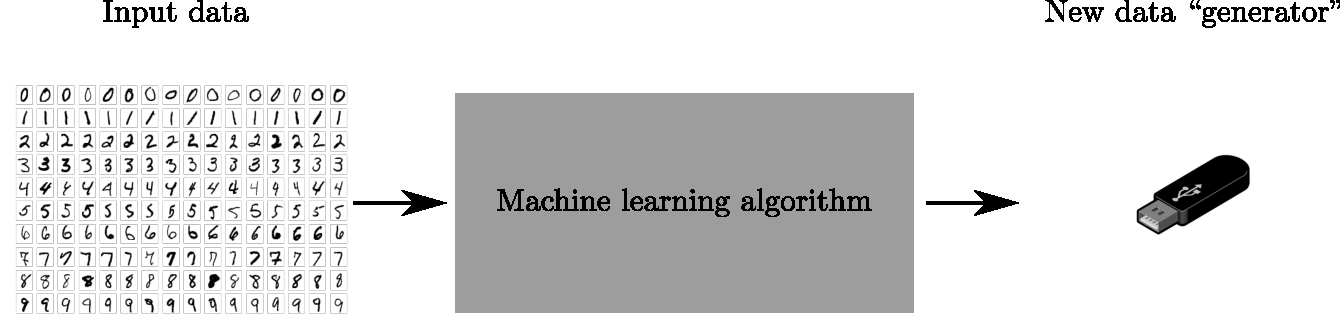
\includegraphics[width=\linewidth]{../figures/MNIST_ML.pdf}
    \end{center}
    \caption{Flow chart of the machine learning process.}
    \label{fig:MNIST_ML}
\end{figure}

You are not required to do this as part of your task this week, but if you are interested in learning about how a Restricted Boltzmann machine can learn MNIST data, you are encouraged to see the \texttt{MNIST} folder. It contains a \texttt{python} script to load MNIST data. There also exists another good database for machine learning algorithm benchmarks called the ``Bars and Stripes'' database. In the \texttt{BarsAndStripes} folder, there is a \texttt{python} script for loading this data.  

\subsection*{Chemistry \& physics motivation?}

Why are machine learning algorithms important in the context of physics and chemistry? Physicists and chemists are faced with an extremely tough firewall when they want to perform numerical simulations known as ``the curse of dimensionality''; problems we want to solve scale exponentially in terms of computational resources. Picture this: you want to send your friend information about one apple via email. The information may include the apple's color, its taste, if there are bruises and where the bruises are on the apple, etc. You've gathered all the information needed about the apple into a text file that ends up taking up 500Kb of data. You email this to your friend without any problems. 

Now, let's say your friend asks you to send information about 10 different apples. It may take quite a while to document everything, but you have the time to do it. At the end of the documentation process, the file takes up 1GB. You probably can't send it via email any longer, so you send it as a Google-drive link. Now, what about 50 apples? Not only is it going to take an extremely long time to document all of the details about each apple, you can't even store all of this information on a 500GB hard-drive! It turns out that the amount of memory and time to perform this task for $N$ apples is approximately $2^N$ Megabytes and $2^N$ minutes \footnote{$2^{50}$ minutes is about 21421231 \textit{centuries}, and $2^{50}$ Megabytes is 1125899900000 Gigabytes...}.
This is precisely the ``curse of dimensionality'' that physicists and chemists face daily. If we want to simulate things in nature, they typically scale exponentially. Machine learning algorithms can compress these problems we want to solve in such a way that squashes this curse of dimensionality into something much more manageable.

\subsection*{Your tasks} \label{sec:tasks}

This week, you'll train an RBM to learn information about the H$_2$ molecule and Rydberg atoms. This is exactly like the MNIST example that was mentioned previously, but instead of hand-written digits we will use data from a molecule / atoms! See Fig.~\ref{fig:H2_ML}. You'll also see how machine learning algorithms address the aforementioned ``curse of dimensionality''.

\begin{figure}
    \begin{center}
        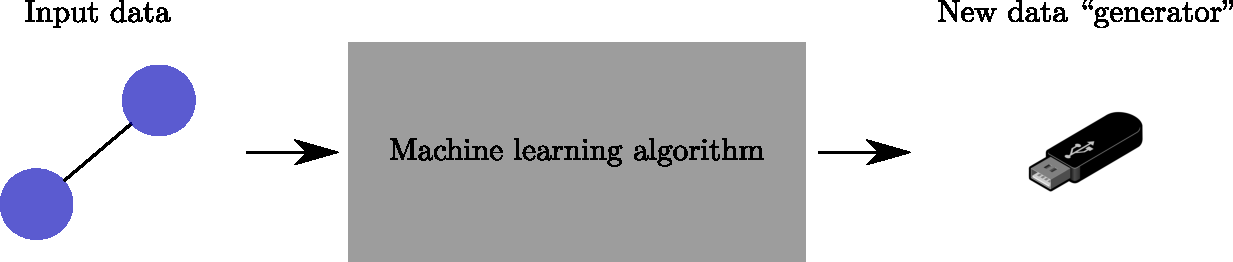
\includegraphics[width=\linewidth]{../figures/H2_ML.pdf}
    \end{center}
    \caption{Flow chart of the machine learning process for this week's tasks.}
    \label{fig:H2_ML}
\end{figure}

\subsubsection*{Task \#1}

In this task, you will train an RBM to reconstruct how the potential energy stored in the H$_2$ molecule varies as the distance between the H atoms changes. You will familiarize yourself with working with RBMs in the process. 

The chemical bond is what forces atoms in a molecule to stay close enough together. If we were to try and take two atoms that are chemically bonded and rip them apart, we would be met with incredible resistance from the retaliation of the bond. On the flip side, there is a repulsive force between atoms that are bonded that ensures that the atoms don't get too close to each other. This balance between the repulsive and attractive forces determines the distance that separates atoms in a chemical bond (called \textit{bond length}). If we were to plot the potential energy stored in a molecule, $E_{bond}$, as a function of the two atoms' separation, $r$, it would look something like the blue or red curve in Fig.~\ref{fig:potential_curve}. It's at the very minimum point on the curves in Fig.~\ref{fig:potential_curve} where the attractive and repulsive forces are in equilibrium with each other.

\begin{figure}
    \begin{center}
        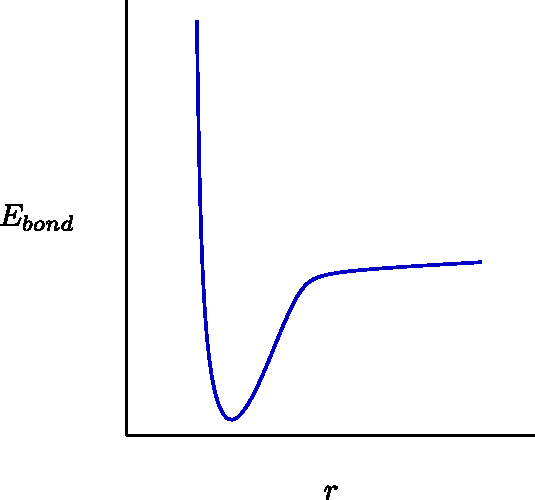
\includegraphics[width=0.4\linewidth]{../figures/potential_energy_curve_vanilla.pdf}
    \end{center}
    \caption{The general form of a molecule's potential energy curve as a function of bond length.}
    \label{fig:potential_curve}
\end{figure}

The code provided to you in \texttt{Task1.ipynb} currently only trains an RBM on H$_2$ data for a specific value of $r$ and calculates the energy from samples generated from the trained RBM. Since we need input data to train the RBM, you're going to need more data for many values of $r$ in order to reproduce a plot that looks like Fig.~\ref{fig:potential_curve}. In the \texttt{H2\_data/} folder you can find the binary input data you need in files called \texttt{R\_<r value>\_samples.txt}. 

$E_{bond}$ can be calculated using the \texttt{energy} function in \texttt{H2\_energy\_calculator.py}\footnote{For more information on how this is calculated, see Ref.      \cite{xiaElectronicStructureCalculations2017}, Eq. (37). We are also using Sections 2.3.1 and 2.3.2 in Ref. \cite{beachQuCumberWavefunctionReconstruction2019} to aid in calculating the energy as a Monte Carlo estimator.}. The \texttt{energy} function takes three arguments: 

\begin{itemize}
    \item \texttt{samples}: the samples generated from the trained RBM.
    \item \texttt{coeff}: parameters required to calculate $E_{bond}$ at a given $r$. All of these parameters for every $r$ value can be found in \texttt{H2\_coefficients.txt} in the \texttt{H2\_data} folder. The file's first column are the $r$ values, and the remaining 7 numbers in each row are the parameters required to calculate the energy. You can just pass these values into the \texttt{energy} function as a \texttt{numpy} array. 
    \item \texttt{RBM\_wvfn}: This is precisely the ``compressed'' entity that contains all of the information about the problem we want to solve. Don't worry too much about the details, but this is required to calculate $E_{bond}$.
\end{itemize}

Here's what we'd like you to do.
\begin{enumerate}
    \item Load in data for all values of $r$ in the \texttt{H2\_data/} folder and train different RBMs for each $r$ value.
    \item With the trained RBM, generate samples from it in order to calculate $E_{bond}$ from those samples. Then, plot $E_{bond}$ for every $r$ and save the image. Does it look like Fig.~\ref{fig:potential_curve}?
\end{enumerate}
Take a second to appreciate what you just did. You successfully used machine learning (an RBM) to learn information about a H$_2$ molecule... Cool! For those wishing to take this a step further, there are other datasets for different molecules. See if you can do the same thing as we did for H$_2$.

\subsubsection*{Task \#2}

Go back to the apples analogy that we talked about earlier for a second. It turns out that Task \#1 is sort of like the 1-apple problem: it's easy to do just by brute force and we didn't really need a machine learning algorithm in the first place. In this task, you'll see the true value of machine learning in physics and chemistry. 

In Task \#1, we gave you plenty of binary input data so that you wouldn't run into any issues. On top of this, learning information about an H$_2$ molecule is actually quite easy for an RBM; we didn't require that many hidden units. In reality, the availability of data is a problem and the difficulty of learning information about certain problems isn't easy. If we were to obtain input data from a real experiment, the experiment may not be stable for long enough to obtain a lot of data. We'll have limited input data to train something like an RBM as a result. Even if we did have a very stable experiment and could obtain as much data as we wanted, we still might be faced with a hard learning problem. So, we'll need a lot of hidden units and the ``compression'' of the original problem won't be as much as we'd hoped.

Your input data for this task will be binary data from 20 atoms. Already, we've hit the ``curse of dimensionality'': the brute force problem at hand scales as $2^N$ in terms of computational resources, where $N$ is the number of Rydberg atoms. To solve this problem via brute force, we'd only be able to go up to around $N = 12$! 

The input data file is \texttt{Rydberg\_data.txt}. To train an RBM on this data, we will look at evaluating the energy \textit{during} training to see how well the RBM is doing and stop the training process once we see that it's done well enough (dubbed the ``learning criterion''). The energy can be calculated using the \texttt{energy} function in \texttt{Rydberg\_energy\_calculator.py}. The learning criteria you'll use is $\vert E_{RBM} - E_{exact} \vert \leq 0.01$ (\textcolor{red}{verify}) (i.e. train the RBM until this is satisfied), where $E_{exact} = -4.00106$. However, don't wait forever for the RBM to try and satisfy the learning criteria. Only wait 5000 training steps (epochs).

Here's what we'd like you to do.
\begin{enumerate}
    \item We've given you a very large dataset in \texttt{Rydberg\_data.txt}. So let's evaluate how ``hard'' the learning problem is (i.e. how many hidden units to reach our learning criteria). Use the entire dataset to determine the minimum number of hidden units required in order to obtain the learning criterion. The ``size'' of the compressed entity that the RBM spits out is the equivalent storage of $20 + n_h + n_h \times 20$ numbers, where $n_h$ is the number of hidden units that you found. How does this compare to $2^{20}$?
    \item Double the number of hidden units determined in the previous question and determine how many data points (i.e. the portion of the full dataset in \texttt{Rydberg\_data.txt}) you need to reach the learning criteria. This will let experimentalists know the minimum amount of data required from their experiment!
\end{enumerate}

Start with the code provided in \texttt{Task2.ipynb}. For those of you interested, we've intentionally left the RBM code in \texttt{RBM\_helper.py} very generic and bare-bones. Use any means necessary to modify this code (or make your own!) and try and improve the results you previously got.

\bibliography{refs}
\bibliographystyle{unsrt}

\end{document}